\section{Test statistic}

To test the level of agreement between the data and the hypothesized value $\mu$, a test statistic $t_{\mu}$ can be defined:
\begin{equation}
    t_{\mu} = -2 ln \lambda (\mu)
\end{equation}
From the definition of $\lambda(\mu)$ in equation~\ref{eq:lambda}, one can see that $0 \le \lambda \le 1$,
and a $\lambda$ with value close to 1 implies good agreement between data and $\mu$.
Thus, larger value of $t_{\mu}$ means the increase of incompatibility between data and $\mu$.
To quantify the level of disagreement, one can calculate the $p$-value as:
\begin{equation}
    p_{\mu} = \int_{t_{\mu, obs}}^{\infty} f(t_{\mu}|\mu) d t_{\mu}
\end{equation}
in which $t_{\mu, obs}$ is the value of test statistic from observed data, 
and $f(t_{\mu}|\mu)$ is the pdf of $t_{\mu}$ under the assumption of hypothesized value $\mu$.
This is a one-side $p$-value with its corresponding observed significance, $Z$, can be defined as:
\begin{equation}
    Z = \Phi^{-1}(1-2p_{\mu})
\end{equation}
The relationship between the $t_{\mu}$, $p$-value and significance $Z$ are depicted in figure~\ref{fig:pvalue_Z}.
When searching for a signal process, such as Higgs boson, the particle physics community tends to claim a discovery
when the rejection of background-only hypothesis has a significance of at least $Z = 5$.

\begin{figure}[!htbp]
\begin{center}
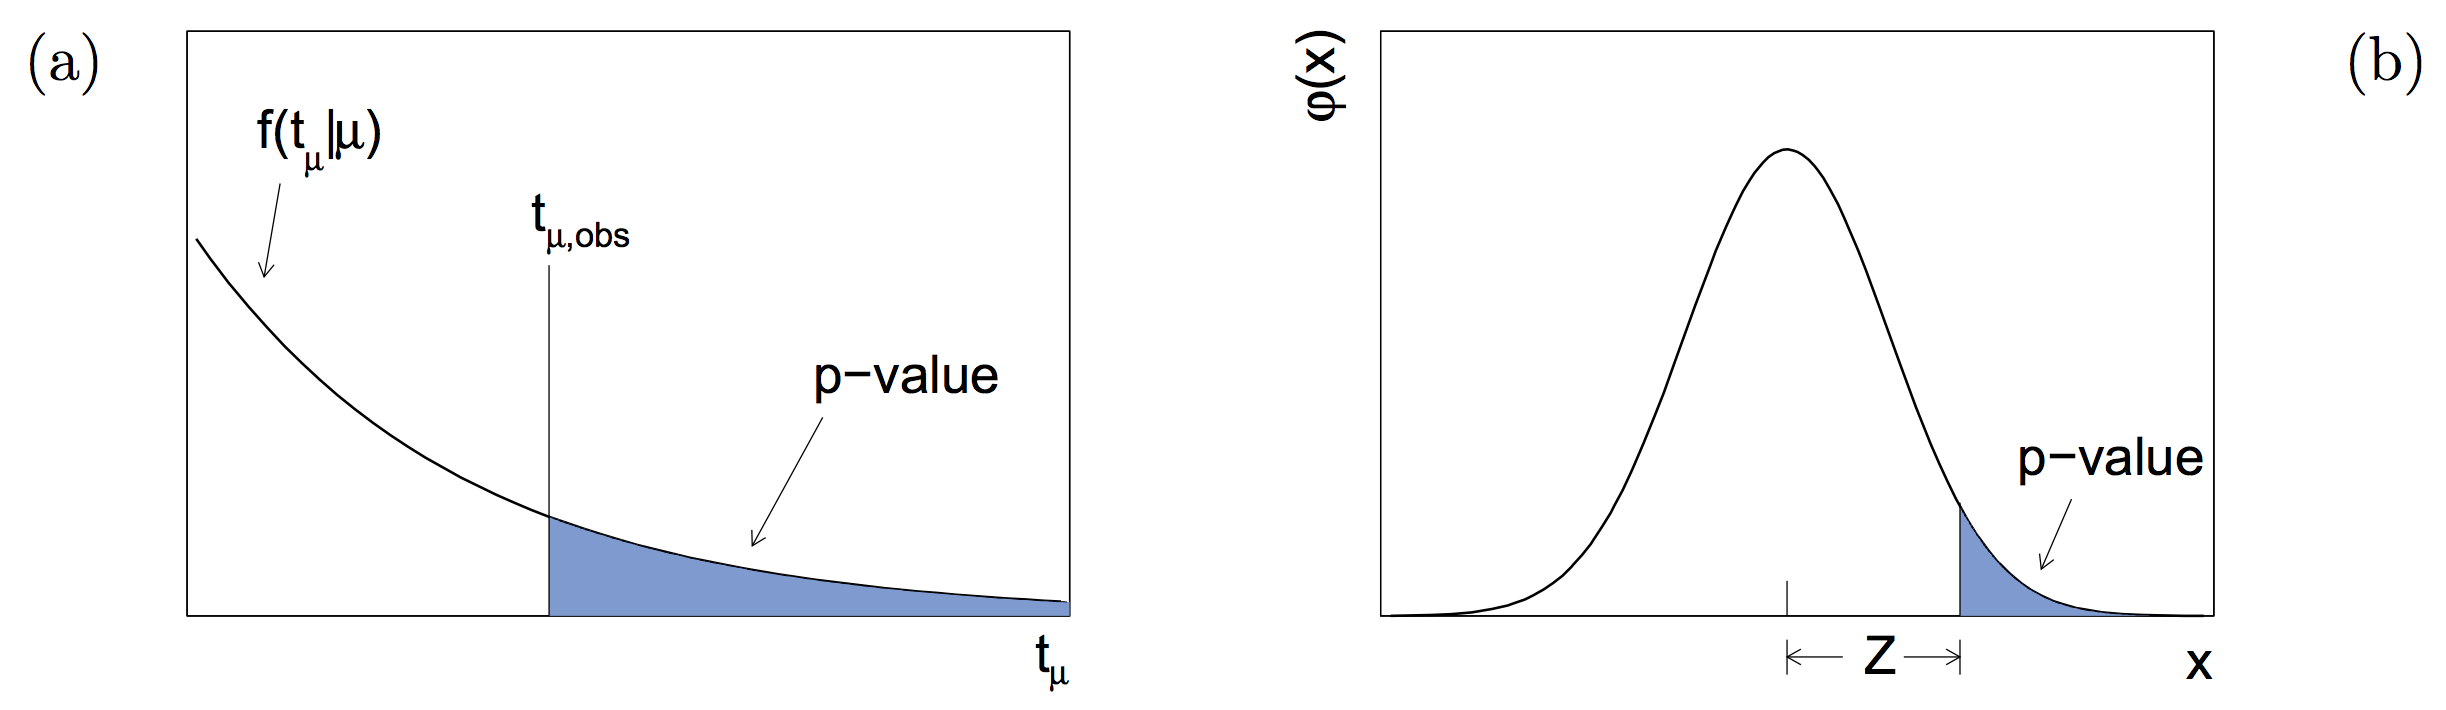
\includegraphics[width=0.42\textwidth]{figures/Statistic/test_statistic_pvalue_Z.png}
\end{center}
\caption{(a) Illustration of the relationship between the observed $t_{\mu}$ and its $p$-value. 
         (b) The relationship between $p$-value and the observed significance $Z$, where $\phi(x)$ is a standard normal distribution.
        }
\label{fig:pvalue_Z}
\end{figure}

In most cases, one assumes that the presence of a new signal can only increase the event rate comparing to the background only model,
then the signal strength $\mu \ge 0$.
And for the case of discovery, the hypothesis of a positive signal strength should be tested against to the background-only (null) hypothesis by using the test statistic called $p_0$:
\begin{equation}
    p_0 = 
    \begin{cases}
        -2 ln(\lambda(0)) &\hat{\mu} \ge 0 \\
        0                 &\hat{\mu} < 0
    \end{cases}
\end{equation}
which corresponds to the $p$-value called $p_0$:
\begin{equation}
    p_0 = \int_{q_{0, obs}}^{\infty} f(q_0|0) d q_0
\end{equation}
to quantify the level of disagreement between the data and the null hypothesis ($\mu = 0$).
